\documentclass[conference,letterpaper,twocolumn]{IEEEtran}
%\usepackage[latin1]{inputenc}
%\usepackage[ansinew]{inputenc}
\usepackage[utf8]{inputenc}

\usepackage{graphicx}
\usepackage{psfrag}
\usepackage{stfloats}
%\usepackage[spanish]{babel}
\usepackage{epsfig}
\usepackage{pifont}
\usepackage{amssymb}
\usepackage{fixltx2e}
\usepackage{amsmath}
\usepackage{rotate}
\usepackage{anysize}
%\usepackage{rotating}
%\usepackage{fancybox}
\usepackage{float}
\usepackage{fancybox}
\usepackage{subfig}

\newcommand{\pig}[1]{\mbox{\boldmath ${#1}$}	}

\newtheorem{Theod}{{\bf Definici\'on}}

\setlength{\oddsidemargin}{5mm}
\setlength{\evensidemargin}{5mm}
\setlength{\topmargin}{4mm}
\setlength{\textwidth}{15cm}
\setlength{\columnsep}{5mm}
\setlength{\textheight}{24cm}





\begin{document}

\title{Double bounded bi-parameter homotopy applied to bipolar/diode circuit simulation}

\author{\authorblockN{H\'ector V\'azquez-Leal, Roberto Casta\~neda Sheissa and Uriel Filobello-Niño }
\authorblockA{Universidad Veracruzana\\
Facultad de Instrumentaci\'on Electr\'onica\\
Xalapa, Veracruz, M\'exico\\
Email: hvazquez@uv.mx}
\and
\authorblockN{\centerline{Arturo Sarmiento-Reyes and Luis Hern\'andez-Mart\'{\i}nez}}
\authorblockA{INAOE\\
Departamento de Electr\'onica\\
Email: jarocho@inaoep.mx}
}

\maketitle

\begin{abstract}

En este trabajo se presenta una homotopía biparam\'etrica con criterio de paro automatizado.
La principal característica de esta homotopía biparam\'etrica es la de tener eje de simetría, doble l{\'i}nea
solución acotante, puntos de inicio y fin arbitrarios y un método para establecer la función biparam\'etrica.  
Además, se ejemplificará el uso del método con un circuito con múltiples puntos de operación.
Finalmente, se discutirá los efectos sobre la homotopía que tiene la elección de diferentes trayectorias para
los parámetros homotópicos.
\end{abstract}
 

\section{Introduction} 

La solución de sistemas de ecuaciones no lineales es una necesidad relevante en diversas áreas de la física; en particular 
en el área de la electrónica la solución de sistemas  de ecuaciones algebraicas no lineales (NAES) permite averiguar el
comportamiento aproximado de los circuitos integrados  antes de ser fabricados, permitiendo así que los diseñadores
rediseñen/optimicen sus circuitos a un bajo costo. El método más utilizado para resolver NAES, es el método de Newton-Raphson (NR), el cual
es de convergencia cuadrática \cite{homo_ogrodzki,cont_quasi}. Sin embargo, debido a que el método NR es de convergencia local \cite{cont_quasi,Schwa_book}, no se puede garantizar que
el método convergerá satisfactoriamente a alguna solución.  Por lo tanto, se ha propuesto los métodos de homotopía, los cuales
tienen mejor convergencia que el método de NR. Asimismo, existe un continuo aumento de complejidad de los circuitos, 
lo que se traduce en una mayor probabilidad de existencia inadvertida de múltiples puntos de operación \cite{netwth_4q}, lo cual
se puede resolver con los métodos de homotopía, ya que éstos métodos son capaces de localizar múltiples soluciones en una misma trayectoria, caso contrario al método de NR, el cual sólo puede localizar una solución por simulación.


\section{Homotopy}


La ecuación de equilibrio de cualquier  circuito se puede formular
a partir del análisis nodal modificado (MNA) \cite{mnaxx}
quedando definida como:

\begin{equation}
{f}({x})={0} \qquad \text{where} \qquad f:\in \mathfrak{R}^n \to  \mathfrak{R}^n 
\label{fx}
\end{equation}
donde $x$ representa a las variables eléctricas del circuito y $n$ es el número de nodos más el número
de elementos no NA compatibles.

Los m\'etodos de homotop\'{\i}a se fundamentan en el hecho de
que las so\-lu\-cio\-nes se encuentran conectadas por una curva, denominada
\emph{curva de so\-lu\-cio\-nes}. 
Para la obtenci\'on de esta curva se agrega
un par\'ametro adicional al sistema de ecuaciones original, lo cual
permite obtener la siguiente ecuaci\'on aumentada:

{\small
\begin{equation}
{H}({f}({x}),\lambda )={0}  \quad \text{where} \quad {H}: \in \mathfrak{R}^n \times  \mathfrak{R} \to \mathfrak{R}^n
\label{homotopia}
\end{equation}}
donde ${H}$ representa la funci\'on de homotop\'{\i}a,
$\lambda$ el par\'ametro de continuaci\'on y
${f}({x})$ la ecuaci\'on original a resolver.

El problema original se convirte en un problema de continuación
num\'erica \cite{homo_richter}, en el que la variable de continuación es el par\'ametro de
homot\'opico $\lambda$. Por lo tanto, ${H}({f}({x}),0)={G}({x})$
donde ${G}: \in \mathfrak{R}^n \to  \mathfrak{R}^n$ es una smooth map el cual tiene una solución
trivial y ${H}({f}({x}),1)={f}({x})$, lo que significa que en $\lambda=1$ se encuentra la solución buscada de ${f}({x})$. 


Un ejemplo  de homotop\'{\i}a est\'a dado por:
\begin{equation}
{H}({f}({x}),\lambda ) =
{f}({x})-(1-\lambda ){f}({x}_{0}) = 0
\label{hexampl}
\end{equation}
Cuando $\lambda =0$, se tiene una soluci\'on conocida {\em a priori}\,
en ${x}_{0}$, usualmente una soluci\'on trivial y en $\lambda =1$ se encuentra la soluci\'on
de la ecuaci\'on ${f}({x})=0$. 

\section{Multiparameter Homotopy}


La homotop\'{\i}a multiparam\'etrica agrega m\'as de un par\'ametro homot\'opico a la ecuación de equilibrio \cite{homo_DWolfMulti}.
Escencialmente tiene un comportamiento similar al de las homotopías uniparametricas, ya que
tiene una soluci\'on trivial cuando los par\'ametros homotópicos tienen un valor de 0
y se localiza la solución de $f(x)$ cuando los parámetros homotópicos alcanzan un valor de 1.
La funci\'on de homotop\'{\i}a
multiparam\'etrica se puede representar como:

\begin{equation}
{H}({f}({x}),\lambda_1,\lambda_2,...,\lambda_k)=0
\end{equation} 
donde $\lambda_1,\lambda_2,...\lambda_k\in[0,1]$, $k$ es el n\'umero de par\'ametros homot\'opicos
y  $x$ es representa los voltajes nodales y corrientes de elementos no-NA compatibles.


Por un lado, las homotopías multiparametricas \cite{homo_DWolfMulti} se han propuesto con la finalidad
de evadir fork bifurcations, singularidades, entre otros problemas que se pueden dar con las trayectorias
homotópicas. Por otro lado, la homotop\'{\i}a multiparam\'etrica aplicada a circuitos se puede interpretar como la
deformaci\'on de un circuito no lineal en un circuito simplificado de solución trivial,
de tal forma que al barrer los par\'a\-me\-tros homot\'opicos, se va transformando el circuito
simplificado hasta coincidir con el circuito no lineal original.
Por lo tanto, este tipo de procedimiento garantiza una suave convergencia
a la soluci\'on final.
Dicha transformación circuital es de amplio inter\'es pues es posible
crear homotop\'{\i}as {\it ad hoc} para la soluci\'on de circuitos caracterizados
por no linealidades espec\'{\i}ficas, como circuitos compuestos por dispositivos tales como:
transistores MOS/Bipolares, memristores, nanotubos, entre otros.
Es posible aplicar homotop\'{\i}as multiparam\'etricas a los modelos
de los dispositivos con el objetivo de {\it linealizar} el circuito justo en inicio de la trayectoria
homotópica, devolviendole suavemente su estado original (no lineal) conforme los parámetros homotópicos llegan
al valor de 1. Finalmente, el trazado de la trayectoria homotópica
 inicia con los parámetros homotópicos en cero donde la soluci\'on es trivial
y termina cuando los parámetros alcanzan el valor de 1 donde la solución es el punto de operación del circuito, sin embargo, 
la forma de la trayectoria intermedia $[0,1]$ para los parámetros homotópicos es aun un tema que se abordara
mas adelante en este artículo.

\section{homotopía biparamétrica doblemente acotada}

Es posible formular una homotopía multiparametrica con criterio de paro, utilizando
la homotopía polinomial doblemente acotada [xxx] cuya formulación es:

\begin{equation}
{
\begin{array}{l}
{H}({f}({x}),\lambda )=QP - W {f}({x})^2
\end{array}}
\label{homotopiaP}
\end{equation}

where $Q=\lambda(\lambda-a)$,  $P=(x-x_i)(x-x_f)$, $W=C(\lambda_1-a/2)^2$, $\lambda_1$ is the homotopy parameter, $a$ is a constant that represents the separation between solution lines, $x_i$ is the initial point, $x_f$ the final point, and $C$ an arbitrary constant.


Ahora se introduce un segundo parámetro homotópico de tal modo que la homotopía se reformula como:

\begin{equation}
{\small
\begin{array}{l}
{H}({f}({x}),\lambda_1, \lambda_2 )=QP - W {f}({x},\lambda_2)^2
\end{array}}
\label{homotopiaPx1}
\end{equation}

donde $Q=\lambda_1(\lambda_1-a)$, ${f}({x},\lambda_2)$ representa la inserción del segundo parámetro homotópico $\lambda_2$ dentro de la ecuación de equilibrio ${f}({x})$, $P=(x-x_i)(x-x_f)$ y $W=C(\lambda_1-a/2)^2$.

El método MNA establece que existe un vector estimulo, el cual contiene la contribución
de  las fuentes de corriente independientes, las fuentes de corriente y voltaje no lineales. 
En este trabajo se considerará el vector estimulo como la suma de dos vectores: uno lineal $i_{lin}$ y otro no lineal $i_{nlin}$.
Además, éste método es similar el análisis nodal, con la diferencia fundamental de
considerar la corriente de rama de los
elementos no NA-compatibles como variables adicionales y sus correspondientes
relaciones de rama como ecuaciones adicionales a la ecuación de equilibrio. La nuevas
variables (corrientes) aparecen en le ecuación de equilibrio como incógnitas adicionales.

\begin{equation}
\left[ \begin{array}{c}
\text{ \it GMNA}
\end{array} \right]
\left[ \begin{array}{c}
{v} \\
{i} \\
\end{array} \right]
=
\left[ \begin{array}{c}
{i_{lin}}
\end{array} \right]
+
\left[ \begin{array}{c}
{i_{nlin}}
\end{array} \right]
\end{equation}
donde {\it GMNA} representa la matriz contribuciones de las conductancias lineales y relaciones de rama de los elementos no-NA compatibles,
${v}$   representa los voltajes de  los nodos del circuito, ${i}$  representa las corrientes de los elementos no-NA compatibles, ${i_{lin}}$ representa las contribuciones
al vector estimulo de todas las fuentes de corriente independientes, y de las caídas de potencial en las fuentes de voltaje independientes, y finalmente ${i_{nlin}}$ representa todas las contribuciones de las fuentes de voltaje y de corrientes no lineales.

El vector ${i_{nlin}}$ contiene las contribuciones de las relaciones de rama
de los elementos no lineales (resitores no lineales).
En un circuito con transistores bipolares el modelo de Ebers-Moll contiene
diodos cuyo modelo m\'as simple es una fuente de corriente no lineal la cual depende exponencialmente de la caída de potencial del diodo. Por lo tanto, la contribución  de la fuente no lineal de corriente a la ecuación se colocará
directamente en la parte no lineal del vector  ${i_{nlin}}$.

Cuando se realiza la deformación del parámetro homot\'opico desde cero hasta uno, lo que se esta haciendo es resolver
inicialmente un problema de solución trivial, continuando con una deformación continua que gradualmente
aumenta la no linealidad de la función homot\'opica $H(f(x),\lambda)$ hasta que en $\lambda=1$, $H(f(x),\lambda)$ es igual a $f(x)=0$.
Asimismo, al agregar el par\'ametro homot\'opico  a la ecuación de equilibrio se debe buscar que la trayectoria homot\'opica sigua una trayectoria lo m\'as suave posible; esto se puede lograr multiplicando $\lambda$ por el vector ${i_{nlin}}$, lo cual es equivalente a multiplicar el parámetro homotópico por las relaciones
de rama no lineales de los componentes del circuito;
Ésto con la finalidad
de suprimir las no linealidades de la ecuación de equilibrio justo en $\lambda_2=0$. Por lo tanto, la función homotópica multiparametrica propuesta en este trabajo es:

\begin{equation}
{\small
\begin{array}{l}
H(f(x),\lambda_1, \lambda_2 )=QP - Wf(x,\lambda_2i_{nlin})^2
\end{array}}
\label{homotopiaPx3}
\end{equation}
donde $Q=\lambda_1(\lambda_1-a)$, $P=(x-x_i)(x-x_f)$ y $W=C(\lambda_1-a/2)^2$. Besides, the
multiparameter homotopy can be expressed in general way as (using $a=1$):

{\small
\begin{displaymath}
{H}(\cdot)= \left\{\begin{array}{rl}
f(x^*)=0 & \textrm{for  $\lambda_1=1, \lambda_2=1$ and $x=x^*$}\\
P=0 & \textrm{for $\lambda_1=0.5$ and $\lambda_2=0$}\\
f(x^*)=0 & \textrm{for $\lambda_1=0, \lambda_2=1$ and $x=x^*$}
\end{array}\right.
\end{displaymath}
}
donde $P=(x-x_i)(x-x_f)$ y la función homotópica depende de ${H}({f}({x}),\lambda_1,\lambda_2{i_{nlin}})$.



La función homot\'opica ${H}$ es una función de $n+2$ variables con $n$ ecuaciones, donde $n$ es igual al n\'umero total de nodos
mas el n\'umero de elementos no-NA compatibles. Por lo tanto es necesario agregar una ecuación extra con la finalidad
de poder utilizar las técnicas convencionales de trazado de trayectorias homot\'opicas\cite{homo_allgower}. 
La ecuación es una función de $\lambda_1$ y $\lambda_2$ la cual se denominará función multiparametrica $M(\lambda_1,\lambda_2)=0$.
Dicha ecuación debe tener dos puntos obligados de cruce ${\lambda}_i=[\lambda_1,\lambda_2]=[0.5,0]$ y ${\lambda}_s=[\lambda_1,\lambda_2]=[1,1]$. De tal modo que ${\lambda}_i$ es el punto donde la solución del circuito es trivial ($x_i$) y  ${\lambda}_s$
es el punto donde la solución de ${H}$ es exactamente la solución buscada de la ecuación de equilibrio ${f}({x}_s)=0$.
La excursión de $\lambda_1$ inicia en 0.5 ya que el eje de simetría
se establece en $\lambda_{sym}=0.5$. Sin embargo, los puntos intermedios de la trayectoria homotópica $\lambda_1-\lambda_2$ no están definidos y juegan un papel
importante en la suavidad de la trayectoria homot\'opica completa. En este trabajo se propone la siguiente ecuación como la función multiparametrica:

{
\begin{equation}
\begin{array}{c}
M(\lambda_1,\lambda_2)=-\lambda_{{1}}+\\ { \left( \lambda_{{2}}+{\frac {B \left( - 1+A \right) }
{AB+ 1- 2A}} \right) \over  \left( -{\frac { \left( - 1+ 2\,
A- B \right) \lambda_{{2}}}{AB+ 1- 2A}}+ 2\,{\frac {B
 \left( - 1+A \right) }{AB+ 1- 2A}} \right) }
\end{array}
\label{homotopiaPx4}
\end{equation}
}
donde $[\lambda_1,\lambda_2]=[A,B]$ es el punto donde cruza la curva de la funci\'on  $M(\lambda_1,\lambda_2)$,
tal como se muestra en la figura \ref{curvasl}(a).

\begin{figure}[hbtp]
\psfrag{o}{$\lambda$}
\centering
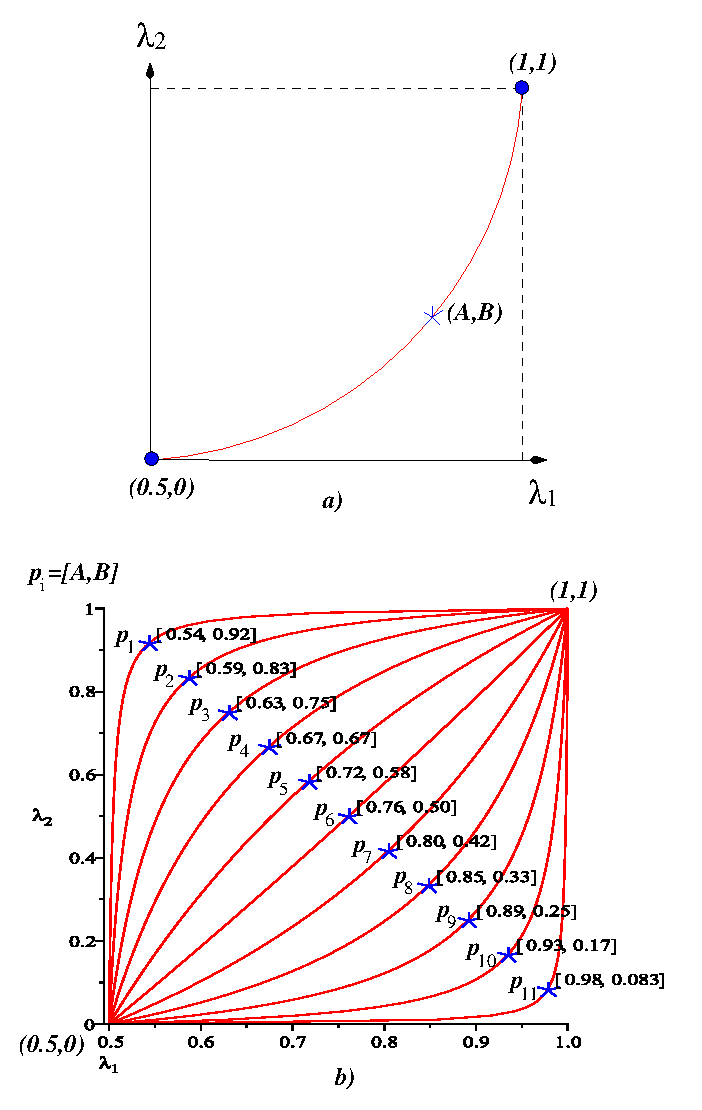
\includegraphics[scale=0.6]{fig/curvasl.eps}
\caption{Trayectoria  de $M(\lambda_1,\lambda_2)=0$ para diferentes puntos $p=[A,B]$}
\label{curvasl}
\end{figure}




En resumen, la homotopía doblemente acotada tiene las siguientes características:

\begin{itemize}
\item Punto de inicio ($\lambda_i$). For $\lambda_1=0.5$ and $\lambda_2=0$ the solution of $H^{-1}(0)$ is known ($x_i$). 
\item Rama simétrica 1. For $\lambda_1=1$ and $\lambda_2=1$, ${H}({f}({x}),1,1)={f}({x})$. Means that at $\lambda_1=1$ and $\lambda_2=1$ all the solutions for ${f}({x})$ are located.
\item Rama simétrica 2. For $\lambda_1=0$ and $\lambda_2=1$, ${H}({f}({x}),0,1 )={f}({x})$. This means that at $\lambda_1=0$ and $\lambda_2=1$ all the solutions for ${f}({x})$ are located.
\item Punto final ($\lambda_f$). For $\lambda_1=0.5$ and $\lambda_2=0$ the solution of $H^{-1}(0)$ is known ($x_f$). 
\end{itemize}


El parámetro homotópico $\lambda_2$ no interfiere directamente con la formulación homotópica, sólo afectando la ecuación de equilibrio $f(x)$ y agregando una ecuación extra al sistema, por lo tanto,
el resto de las propiedades de esta homotopía multiparametrica concide con la homotopía reportada en \cite{xxx1}, como lo es: ramas simétricas, eje de simetría, punto de inicio
y punto final de la trayectoria homotópica y criterio de paro. Ahora se discutirá una ejemplo de aplicación de la homotopía propuesta.


\section{Study case: Circuit with bipolar transistors and a diode}


A circuit with bipolar transistors and a diode was reported in \cite{homo_tadeusiewicz} and  \cite{homo_yamamurawise}, it was solved using piecewise methods. Then, in \cite{homo_yamamura}, the circuit was resolved using modified fixed point Homotopy. This circuit has 3 operating points. The Ebers-Moll is used for all the transistors. The equation for the model is given as:

\begin{displaymath}
\left[ \begin{array}{c}
i_{D_E} \\
i_{D_C}
\end{array}\right] =
\left[ \begin{array}{cc} 1  & \alpha_R \\
\alpha_F & 1 \\
\end{array}\right] \left[ \begin{array}{c}
10^{-9}(e^{(40v_{be})} - 1) \\
10^{-9}(e^{(40v_{bc})} - 1)
\end{array}\right]
\end{displaymath}

As for the diode, the model is:

\begin{displaymath}
i_d=10^{-9}(e^{40u} - 1)
\end{displaymath}

\begin{figure}[hbtp]
\centerline{
\epsfxsize=75mm
\epsffile{yamamura/diotran.eps}
}
\caption{Circuit with bipolar transistors and a diode.}
\label{yamamuracircuito}
\end{figure}

First, the equilibrium equation is formulated using the modified nodal analysis with the result of a system having 14 equations and 14 variables. The circuit is shown in figure \ref{yamamuracircuito}.


Now, DBH is applied to solve the circuit; the Homotopy formulation is expressed as follows:


\begin{displaymath}
{\small
\begin{array}{r}
H_1(\cdot)=Q(v_1-13)(v_1+13)+ W f_1^2=0\\
H_2(\cdot)=Q(v_2-13)(v_2+13)+ W f_2^2=0\\
\vdots \qquad \\
H_{13}(\cdot)=Q(v_{13}-13)(v_{13}+13)+ W f_{13}^2=0\\
H_{14}(\cdot)=Q(I_E-13)(I_E+13)+ W f_{14}^2=0\\
M(\lambda_1,\lambda_2)=0
\end{array}}
\end{displaymath}


where $Q=\lambda_1(\lambda_1-1)$, $W=C(\lambda_1-0.5)^2 $, the constant value $C=1$, the bounding lines are $[\lambda_1,\lambda_2]=[0,1]$ and $[\lambda_1,\lambda_2]=[1,1]$, las ecuaciones nodales $f$ dependen de $(v_1,v_2,\hdots,v_{13},I_E,\lambda_2i_{nlin})$ and the initial point $x_i$ for the Homotopy path is selected as shown in figure \ref{yamaie}(c).

Se simula el circuito con una técnica de trazado convencional como las mostradas en \cite{homo_allgower}.
Con la finalidad de mostrar los efectos de la selección especifica de una función multiparametrica $M(\lambda_1,\lambda_2)=0$, se eligieron
3 casos particulares: $p_1$ (trayectoria $M_1$) y $p_{11}$ (trayectoria $M_{11}$), por representar los 2 casos de trayectorias extremas y $p_6$ (trayectoria $M_6$)
por representar una relación de dependencia lineal (aproximada) entre $\lambda_1$ y $\lambda_2$ (ver figura \ref{curvasl}(b)). 
En la tabla \ref{yamamuracircuitosoluc} se resumen los resultados de trazar las 3 trayectorias homotópicas respectivas
a cada función multiparametrica a partir del mismo punto de inicio $x_i$, los cuales se discuten a continuación:

\begin{itemize}
\item Todas las trayectorias ($M_1$, $M_6$ y $M_{11}$) presentaron un doble acotamiento ($\lambda_1=0$ y $\lambda_1=1$ )  y eje de simetría $\lambda_{sym}$.
\item Se trazó exitosamente la rama simétrica correspondiente a la línea solución $\lambda_1=1$.
\item En cada caso se localizó los 3 puntos de operación (ver tabla \ref{yamamuracircuitosoluc1}).
\item El número de turning points (TP) es  11 para las tres trayectorias.
\item $p_1$ y $p_{11}$ presentan un menor número de iteraciones (Iter) para completar el trazado de la trayectoria que la
trayectoria de en medio $p_6$. Además, $p_{11}$ presenta el  menor número de iteraciones, donde $p_{11}$ representa aproximadamente
el comportamiento (cualitativo) donde primero se barre $\lambda_1$ desde 0.5 hasta 1 y luego $\lambda_2$ se barre desde 0 hasta 1.
\item El punto final de las trayectorias $M_1$ y $M_{11}$ es el mismo. Esto implica
que las trayectorias extremas puede ser similares indistintamente de que parámetro se
barra primero ($\lambda_1$ o $\lambda_2$).
\item El punto final de la trayectoria lineal $M_{6}$ difiere de las otras dos trayectorias ($M_1$ y $M_{11}$).
Este resultado implica que es posible afectar la trayectoria homot\'opica dependendiendo
de la selección realizada para la función paramétrica $M$.
\end{itemize}

El mismo número de soluciones y turning points pero diferente número de iteraciones significa que 
las 3 trayectorias tienen aspectos simulares como se presentada en la figura \ref{yamaie}. Sin embargo,
el número de iteraciones diferente sugiere que aunque las 3 trayectorias cruzan aproximadamente por los mismos pliegues de la ecuación
de equilibrio con ligeras diferencias en la localización exacta de los turning points y que cambia el valor del radio de curvatura correspondiente tanto para los puntos de retorno como para los puntos de rebote en las soluciones (ver figura \ref{yamaie}). Finalmente, la trayectoria $M_6$ tiene un mayor número de iteraciones
y un punto final diferente (que los de $M_1$ y $M_{11}$) lo que sugiere que es posible afectar
la trayectoria homotópica con la selección de una $M$ apropiada. En el caso de estudio presentado
en este trabajo la función  $M$ óptima puede ser cualquiera de los 2 casos extremos de funciones paramétricas $M_{1}$ o $M_{11}$.
En \cite{homo_MOS} se propone una homotopía multiparametrica, la cual sólo localiza un punto de operación por simulación,
no contiene un criterio de paro automatizado, ni líneas solución que acoten la trayectoria, por lo tanto,
en este sentido la homotopía propuesta en el presente trabajo presenta ciertas ventajas. 


Finalmente, se implemento una función  multiparametrica polinomial ($M_{12}$): 
{\small
\begin{displaymath}
\begin{array}{c}
M(\lambda_1,\lambda_2)=-\lambda_2+ 98.09523810\lambda_1^3- \\ 221\lambda_1^2+ 161.8333333\lambda_1-37.92857143
\end{array}
\end{displaymath}
}
La función multiparametrica $M_{12}$ se muestra en la figura \ref{yamaie}(g) y su trayectoria
homotópica correspondiente en las figuras \ref{yamaie}(i) y \ref{yamaie}(j). Se puede notar como
el numero total de iteraciones fue menor que el alcanzado con las funciones parametricas: $M_1$, $M_6$ y $M_{11}$
e inclusive el punto final de la trayectoria es diferente. Esto confirma que la elección de la función
multiparametrica puede jugar un rol importante en el desempeño de la función bi-parametricas doblemente acotada.


En \cite{homo_MOS}
se presentan simulaciones de circuitos de hasta 8489 transitores, lo que se intentará alcanzar en una futura  continuación
de este trabajo de investigación.




\begin{figure*}[hbtp]
\centerline{
\epsfxsize=105mm
\epsffile{fig/yamamu.eps}
}
\caption{Homotopy trajectory for $v_2-\lambda_1$}
\label{yamaie}
\end{figure*}



\begin{table*}[htbp]
{\small
\center{
\hspace{-4mm}
\begin{tabular}{||c|c|c|c|c|c|c|c|c|c|c|c|c|c|c|c|c||}
\hline\hline
Points & Iter & TP &$v_1$ & $v_2$ & $v_3$ & $v_4$ & $v_5$ & $v_6$ & $v_7$ & $v_8$ & $v_9$ & $v_{10}$& $v_{11}$ & $v_{12}$ & $v_{13}$ & $i_E$  \\ \hline
$x_i$ & - & - &+13 & +13& +13& -13& +13& +13& +13& +13& +13& +13& +13& +13& -13& -13  \\ \hline
$x_f(M_1)$ & 16669 & 11&+13& +13& +13& -13& +13& +13& +13& +13 & +13& +13&+13&+13&-13&+13   \\ \hline
$x_f(M_6)$ & 17063 &11 & +13 & -13 & +13 &-13& +13&  +13& +13& +13& +13& +13& +13& +13& -13& +13     \\ \hline
$x_f(M_{11})$ & 16508 &11 &+13& +13 & +13& -13& +13& +13& +13&+13& +13& +13& +13& +13& -13 &+13  \\ \hline 
$x_f(M_{12})$ & 16112 &11 &+13& +13 & -13& -13& +13& +13& +13&+13& +13& +13& +13& +13& -13 &+13  \\ \hline \hline
\end{tabular}
}
}
\caption{Puntos extremos de las 3 trayectorias homotópicas, considerando $\lambda_1=0.5$ and $\lambda_2=0$.}
\label{yamamuracircuitosoluc}
\end{table*}


\begin{table*}[hbtp]
{\small
\center{
\hspace{-4mm}
\begin{tabular}{||c|c|c|c|c|c|c|c|c|c|c|c|c|c|c||}
\hline\hline
Sol & $v_1$ & $v_2$ & $v_3$ & $v_4$ & $v_5$ & $v_6$ & $v_7$ & $v_8$ & $v_9$ & $v_{10}$& $v_{11}$ & $v_{12}$ & $v_{13}$ & $i_E$ \\ \hline
$S_1$ &  12 & 5.995 & 0.085 &0.368 &0.712 &0.436 &0.390 &0.699 &11.635 &0.4e-5 &0.039 &0.039 &0.321 &-0.0089 \\ \hline
$S_2$ & 12 & 0.883 & 0.278 &0.590 &0.631 &0.812 &0.315 &1.074 &11.647 &0.4e-5 &0.039 &0.039 &0.321 &-0.0100 \\ \hline
$S_3$ & 12 & 0.405 & 0.366 &0.685 &0.349 &6.796 &0.070 &7.038 &11.839 &0.4e-5 &0.039 &0.039 &0.321 &-0.0085 \\ \hline \hline
\end{tabular}
}
}
\caption{Three Operating points (solutions) found at $\lambda_1=1$ and $\lambda_2=1$}
\label{yamamuracircuitosoluc1}
\end{table*}


\section{Conclusions}

En el presente trabajo se demostró que es posible crear una homotopía biparametrica con doble acotamiento,
la cual presentó doble línea solución, eje de simetría, punto de inicio y punto final para su trayectoria.
Se mostró un esquema de selección de la trayectoria homotópica el cual resultó ser óptimo para la trayectoria $M_{11}$
en el caso de estudio presentado.


\bibliographystyle{amsplain}
\bibliography{carta}

\end{document}
